\documentclass[11pt,
  oneside,openany,    % for one-sided printing and screens
  %parskip=half,      % enable if you want paragraphs separated by vertical spacing instead of indents
  %draft              % enable to compile faster and test layout
]{scrreprt}

% Settings
\usepackage[english]{babel}
\usepackage[utf8]{inputenc}
\usepackage{geometry}
\usepackage{microtype}
\usepackage[all]{nowidow}
\usepackage[bsc,             % for Bachelor's Thesis titlepage
            %project,        % for Master's Project titlepage
            claim,isec]{isecthesis}
\addtokomafont{disposition}{\rmfamily}

% <INSERT YOUR CUSTOM MACROS AND PACKAGES HERE>

% Useful packages for complex content:
\usepackage{amsmath,amsfonts,amssymb} % typesetting math
\usepackage{tikz}                     % typesetting diagrams, figures, ...
%\usepackage{pgfplots}                % typesetting plots and diagrams (via TikZ)
%\usepackage{siunitx}                 % typesetting SI-units and formatted numbers
\usepackage{listings}                 % typesetting source code
%\usepackage{booktabs,multirow}       % utils for complex/beautiful tables
\usepackage{subcaption}               % placing multiple subfigures in a figure
\usepackage{tabularx}

% Useful utils:
%\usepackage{todonotes}               % add ToDo markers (\todo{...})
%\usepackage{xspace}                  % define macros that don't eat the following space (add \xspace at the end)
%\usepackage[section]{placeins}       % prevent figures from floating into the wrong section (\FloatBarrier)

% Bibliography, referencing, and indexing
\usepackage{csquotes}                 % typesetting \enquote{text in quotes} correctly
\usepackage[backend=biber,
            % style=alphabetic,
            % minalphanames=3, maxalphanames=4,
            maxbibnames=20]{biblatex} % to generate the bibliography
\addbibresource{thesis.bib}           % name of the bib-file

\usepackage[hidelinks]{hyperref}      % clickable links (but hide color frames around links)
\usepackage{cleveref}                 % named references (\Cref{chap:introduction}, ...)

% \usepackage[toc,acronym,style=long3col]{glossaries} % List of acronyms and symbols  (optional)
% \makenoidxglossaries
%
% \newacronym{aes}{AES}{Advanced Encryption Standard}
% \newglossaryentry{xor}{name={\ensuremath{\oplus}}, sort=xor,
%                        description={exclusive-or (\textsc{Xor})}}
% <INSERT YOUR GLOSSARY ENTRIES HERE (or \input{} a dedicated file) >

\usetikzlibrary{shapes.geometric, arrows}

\lstset{
  frame=tb,
  backgroundcolor=\color{gray!10},   
  commentstyle=\color{black!50!green},
  keywordstyle=\color{blue},
  numberstyle=\tiny\color{gray},
  stringstyle=\color{red!58!black!82},
  basicstyle=\ttfamily\footnotesize,
  numbers=none,
  breakatwhitespace=false,         
  breaklines=true,                 
  keepspaces=true,                                    
  showspaces=false,                
  showstringspaces=false,
  showtabs=false,                  
  tabsize=2,
  captionpos=b,
  columns=flexible
}


\begin{document}

%--- INSERT INFORMATION FOR TITLEPAGE ------------------------------------------

% Your name + previous academic degrees:
\thesisauthor{Gergö Kranz}

% Title of your thesis:
\thesistitle{AndroGUARD: Mitigation of\\Sensor Fingerprinting on Android}

% Date of completion:
\thesisdate{February 2025}

% Supervisor:
\supervisortitle{Supervisor} % or Supervisor
\supervisor{%
  Gerald Palfinger
  \smallskip

  Institute of Information Security\\
  Graz University of Technology
}

% Name of your degree programme according to your curriculum
\curriculum{Software Engineering and Management}



%--- FRONT MATTER --------------------------------------------------------------

\printthesistitle

\chapter*{Abstract}

Sensor fingerprinting is a technique that enables the unique identification of users based on specific characteristics of the sensors in their devices. 
This unique fingerprint has the potential to deanonymize mobile devices and track them.

In this thesis, we look into the fingerprintability of the sensors in an Android device.
Our main contribution is the implementation of the masking of the built-in sensor error to decrease Android fingerprinting efficiency.
The built-in factory calibration error refers to the slight inconsistencies and inaccuracies introduced during the manufacturing and factory calibration process of sensors. 
These errors are characteristic to each device and remain constant over its lifetime, providing a consistent yet unique signature that can be used for fingerprinting.
We examine proposed mitigation techniques and implement our solution to mitigate fingerprinting, that can be applied to Android application packages.
Our approach adds random noise to the original sensor values, before they are passed down to the function handling them.
With the help of the Android Application Patching Pipeline we can apply our patch to any compatible Android app.
We evaluate how varying noise levels affect the effectiveness of our obfuscation technique, finding that while increased noise enhances privacy by reducing fingerprintability, it also compromises the usefulness of sensor values.
We conclude that by adding random noise we mask the consistency of the built-in factory error to make sensor fingerprinting more complicated.

\paragraph{Keywords:}
Android API $\cdot$
Sensor Fingerprinting $\cdot$
Privacy $\cdot$
Protection

\cleardoublepage
% \tableofcontents  % optional

\chapter{Introduction}
\label{chap:introduction}

Through the utilization of the Android API, applications can access a wide array of device-specific information essential for their operation.
While this functionality is designed to support app performance by providing crucial data, it also exposes certain device features and configurations that, when combined, can be used to uniquely identify users based on the specific characteristics of their device and system settings \cite{DBLP:conf/IEEEares/PalfingerP20}.
The practice of tracking Android users via device fingerprinting, without their knowledge and explicit consent, raises significant privacy and security concerns.
This method allows users to be tracked across multiple applications and services, often without their awareness, which constitutes a clear infringement of privacy.

Advertisers frequently employ fingerprinting techniques to compile detailed user profiles for targeted advertising.
However, malicious actors may exploit the same fingerprinting information for nefarious purposes, such as orchestrating tailored phishing attacks or deploying malware optimized for the user's specific device configuration.
Moreover, the collection of data from the API could reveal a substantial amount of sensitive information.
When such data is aggregated, it may lead to a variety of fraudulent activities, leading to both security risks and privacy violations.

Fingerprints can be based on various characteristics of the software and hardware configuration of the device, providing a way to distinguish it from other devices.
Some of the used information is based on the system properties of the device, network, or device configuration by the user \cite{DBLP:journals/popets/KurtzGBRF16}. 
These properties can include details about the operating system, kernel version, and runtime parameters \cite{DBLP:journals/access/WuWWLY16}.
Furthermore, details about the Android build version, manufacturer, model, and build number can be included in the fingerprint. 
Additionally, separate hardware components, like camera and speaker, can be uniquely fingerprinted \cite{DBLP:journals/tifs/Li10, DBLP:journals/popets/DasBC18}.

In this thesis, we focus on reducing the fingerprintability of sensors.
Sensor fingerprinting refers to the process of identifying and tracking individual devices based on the unique characteristics and imperfections of their built-in sensors \cite{DBLP:conf/ndss/DeyRXCN14}. 
These imperfections in sensors, exploited for fingerprinting, arise from manufacturing variations, material defects, calibration inaccuracies, and various environmental factors \cite{DBLP:journals/comsur/BaldiniS17, DBLP:journals/popets/DasBC18, DBLP:journals/tifs/ZhangBS21}. 
Android devices, which are equipped with various sensors like accelerometers and gyroscopes are vulnerable to this type of fingerprinting \cite{DBLP:conf/ndss/DasBC16}. 
These sensors, while essential for providing enhanced functionality and user experiences, can inadvertently expose unique error patterns that can be exploited for tracking purposes. 
By focusing on sensor fingerprinting, this thesis aims to explore the methodologies used to extract these unique signatures, assess the potential privacy risks, and implement effective countermeasures to mitigate these risks, thereby enhancing user privacy and security in the Android ecosystem.

Multiple papers have been published on fingerprinting sensors in Android devices by recording their built-in imperfections, which arise from the manufacturing process \cite{DBLP:conf/ccs/DasBC14}. 
These studies demonstrate that the measurement errors inherent in these sensors are unique to each device, creating a distinctive fingerprint \cite{DBLP:conf/ccs/0001ABP18, DBLP:journals/tifs/AmeriniBCMN17}. 
Furthermore, they show that these errors are consistent and stable over the lifetime of the sensor, making them reliable indicators for identifying and tracking individual devices. 
This consistency in sensor errors highlights the potential privacy risks associated with sensor fingerprinting, as it allows for the persistent and unique identification of devices based solely on their hardware characteristics.
While these papers highlighted the problem there is currently no mitigation implemented in Android.
We will address this problem by implementing a possible solution which masks these sensor imperfections.

Our implementation of AndroGUARD builds on suggestions from some of the research papers which covered this issue \cite{DBLP:conf/ndss/DasBC16, DBLP:journals/tifs/AmeriniBCMN17, DBLP:conf/ccs/0001ABP18}. 
To implement and deploy our mitigation we use the Android Application Patching Pipeline (A2P2) \cite{DBLP:conf/IEEEares/Draschbacher23}.
We aim to effectively obfuscate sensor data and prevent the extraction of identifiable information, by integrating the recommended strategy from a reviewed research paper \cite{DBLP:conf/ndss/DasBC16}. 
By introducing random variations to sensor outputs, we can obscure unique error patterns, making it more challenging for adversaries to reliably fingerprint and track devices \cite{DBLP:journals/tifs/AmeriniBCMN17}. 
Our approach not only addresses the vulnerabilities highlighted in the literature but also provides practical solutions to enhance the privacy and security of Android users.

\paragraph{Outline.}
In Chapter \ref{chap:background}, we offer an overview of general fingerprinting techniques. 
Moving forward to Chapter \ref{chap:sensor_fingerprint}, we focus on sensor fingerprinting, where we detail its mechanics, common sensor types targeted, and real-world implications.
Building on this information, in Chapter \ref{chap:methodology} we examine existing countermeasures against fingerprinting, evaluating their effectiveness and limitations to provide context for our proposed solution. 
Chapter \ref{chap:approach} investigates the mitigation concepts presented in prior research, understanding relevant literature for our implementation of the selected mitigation strategy.
Following this, Chapter \ref{chap:implementation} provides a detailed breakdown of the patch creation process, including integration with the A2P2 framework and key functionalities such as the intercept method and noise generation. 
Chapter \ref{chap:evaluation} shifts focus to validating the effectiveness of the patch, detailing the testing methodology, results, and areas for further improvement. 
By highlighting the implications and discussing the limitations of our work, Chapter \ref{chap:disc_and_limits} offers directions for future research.
Finally, Chapter \ref{chap:conclusion} summarizes our findings, reflects on the implications of the project, and outlines directions for future research and development.

% You may want to keep your chapters in separate files ('chapterfilename.tex')
% and include them here using either
%\input{chapterfilename.tex}   or   \include{chapterfilename}

\chapter{Background}
\label{chap:background}
With the help of fingerprinting, users and their habits can be tracked to create personalized profiles of them.
However, tracking users based on the fingerprint of their devices raises various privacy and security concerns \cite{DBLP:conf/ndss/MengZXZZBLTD23}.
While advertisers may use fingerprints to build detailed profiles of users for targeted advertising, malicious actors on the other hand could exploit the information gathered for their targeted attacks. 
For example, they may use the collected data to tailor phishing attempts or deliver malware specific to the user's device configuration.
Detailed fingerprinting could potentially expose a variety of sensitive information that, when combined, may lead to identity theft or other fraudulent activities.
Due to this, users might feel uncomfortable or even violated if they perceive that too much of their personal information is being used without their control.
The practice of extensive fingerprinting may run against data protection regulations such as GDPR, which require explicit user consent for collecting and processing personal data.
In the following, we will explore browser and mobile fingerprinting, focusing on their similarities and differences.

\section{Browser Fingerprinting}
\label{sec:browser_fingerprint}
Browser fingerprinting is a widely known technique, which is frequently exploited to track users across different websites \cite{DBLP:conf/secrypt/PolcakSMHM23}.
By using mainly JavaScript the visited website can access system information like screen resolution or settings set by the user.
These attributes can be combined to create a unique identifier of the device.

\paragraph{Browser Fingerprinting Methodologies.}
\label{par:browser_fingerprint}
Different methods can be applied to fingerprint a browser as shown by \citeauthor{DBLP:conf/ntms/UpathilakeLM15} \cite{DBLP:conf/ntms/UpathilakeLM15}.
Browsers can be fingerprinted by analyzing various browser-specific attributes, such as the browser version, installed fonts, and other identifiable characteristics.
Additionally, HTML5 functionalities, particularly the rendering of text and WebGL scenes via the canvas element, can be leveraged to generate a fingerprint.
By rendering content and subsequently retrieving pixel data from the canvas, a unique identifier based on subtle differences in how the browser displays these elements can be constructed.
This technique allows for the creation of a detailed fingerprint that can be used to distinguish users across sessions.
JavaScript can also be used to create cross-browser fingerprints, which is browser independent and focuses more on the hardware the browser is running on, like screen resolution or networking information.
With the use of JavaScript also sensor data can be accessed to create sensor fingerprints.

\paragraph{Browser Fingerprinting Protections.}
\label{par:browser_fingerprint_protect}
A number of solutions have already been presented in multiple research papers to identify and block fingerprinting efforts, making browsing the internet more private for everyone. 
JShelter \cite{DBLP:conf/secrypt/PolcakSMHM23} blocks the execution of JavaScript to mitigate the gathering of personal data used for fingerprinting to increase browser security.
Another study, PriVaricator \cite{DBLP:conf/www/NikiforakisJL15}, aims to reduce the determinism of browser fingerprints by introducing controlled randomization, thereby mitigating the ability to consistently identify users across multiple visits to the same website.
This approach disrupts the reliability of fingerprinting techniques by making the data less predictable and harder to track.
These research projects disrupt the consistent behavior required by features like adaptive layouts, multimedia rendering, and security mechanisms, leading to broken or degraded functionality. 
To solve this issue FP-Block \cite{DBLP:conf/esorics/TorresJM15} creates a different unrelated fingerprint for the embedded resources to maintain their functionality, but prevent tracking.

\section{Smartphone Fingerprinting}
\label{sec:smartphone_fingerprint}
The concepts underlying browser fingerprinting can similarly be applied in the context of smartphone applications \cite{DBLP:conf/IEEEares/PalfingerP20}. 
Similarly, mobile fingerprinting relies on the extraction of various device specific characteristics, such as the mobile operating system, device model, screen dimensions, app usage data, and other hardware or software attributes, to construct a unique identifier for the device.

A study by \citeauthor{DBLP:conf/www/Gomez-BoixLB18}, about mobile browsers, highlights the differences the distinct behaviors in the absence of plugins like Flash \cite{DBLP:conf/www/Gomez-BoixLB18}.
The analysis covers over 17,000 mobile fingerprints collected, finding that 81\% of these fingerprints are unique. 
The dataset includes a multitude of operating systems, primarily Android devices.
The user-agent attribute is the most distinctive, with over 3,000 unique values, due to detailed information about the device's operating system, version, and browser. 
The study also confirmed that mobile user-agents contain more specific information than desktop user-agents, sometimes indicating modified third-party ROMs.
The canvas attribute, influenced by unique emoji sets from different manufacturers, is the second most distinctive with around 700 unique values.
The study confirms that mobile browser fingerprinting is effective in uniquely identifying devices, due to specific mobile software environment characteristics.

The aforementioned paper primarily focuses on the use of web browsers on mobile devices as a context for fingerprinting; however, it is important to recognize that web browsers are not the only environments in which fingerprinting techniques can be applied.
Fingerprinting can occur in a variety of different contexts, including mobile applications.
In the subsequent paragraphs we will focus on methods used to identify and track users through mobile applications.

There is a novel approach to identify Android devices through fingerprinting methods that bypass the need for user-granted permissions.
It leverages zero-permission identifiers, such as hardware configurations, sensor data, and system settings, which can be accessed without explicit user consent.
By combining these attributes, a fingerprint that uniquely identifies a device across different applications and sessions can be developed.
This technique is highly efficient, requiring minimal computational resources while achieving accurate identification.
The study written about this methodology highlights the significant privacy risks associated with such methods, as they allow tracking of users without traditional permission mechanisms or user awareness \cite{DBLP:journals/access/WuWWLY16}.

In a similar fashion mobile devices can be uniquely identified through their personalized configurations, even without direct access to hardware identifiers.
It was demonstrated that a combination of software and user-specific settings, such as installed apps, language preferences, timezone settings, and network configurations, can be used to create a distinct fingerprint for each device.
This method allows accurate device tracking across different platforms and applications.
The paper that studied this approach raised concerns about privacy, emphasizing that even seemingly benign configurations can reveal a great deal about a user and facilitate tracking without their consent \cite{DBLP:journals/popets/KurtzGBRF16}.

Restricted access to sensitive identifiers is crucial to hinder fingerprinting attempts. 
Android advocates for the responsible use of device information, by blocking access to unique identifiers, like IMEI numbers \cite{android_privacy_10, DBLP:conf/ndss/MengZXZZBLTD23}.
Users have the freedom to review and modify app permissions through system settings, enabling them to manage access to personal information effectively. 
When supported by user education this permission model empowers the owner of the device to take informed decisions about the data they are willing to share with applications \cite{DBLP:conf/icta/NegashS15}.
Despite the current permission system, there remains a significant possibility for fingerprinting through, for instance, the use of sensor values.
Therefore, the following chapter will describe how a permissionless fingerprinting technique can be used to track users without restrictions from the Android operating system and the knowledge of the user.

\chapter{Sensor Fingerprinting}
\label{chap:sensor_fingerprint}
In this thesis, our central focus is the complex problem of sensor fingerprinting applicable to a wide range of Android devices \cite{DBLP:journals/comsur/BaldiniS17}. 
Sensors embedded within smartphones and tablets serve as the foundation for an extensive array of functionalities, spanning from location tracking and environmental monitoring to augmented reality experiences and health tracking applications. 
However, these features introduce potential vulnerabilities related to the misuse of sensor data.
When exploited through fingerprinting techniques, such data can compromise user privacy and security \cite{DBLP:conf/ndss/MengZXZZBLTD23}.

It has been shown by multiple research papers that the built-in error of sensors remains consistent over the lifetime of the device \cite{DBLP:conf/sp/ZhangBS19, DBLP:conf/ndss/DeyRXCN14}. 
This inherent characteristic of sensors, stemming from manufacturing imperfections and the initial calibration, results in a unique and persistent signature that does not change significantly over time. 
Multiple studies \cite{DBLP:journals/popets/DasBC18, DBLP:conf/ndss/DasBC16, DBLP:conf/ccs/DasBC14, DBLP:conf/ccs/0001ABP18} have demonstrated that these discrepancies can be reliably measured and used to fingerprint individual devices, posing a significant threat to user privacy. 
This stability of sensor errors forms the basis for sensor fingerprinting techniques, highlighting the need for effective countermeasures to disrupt these patterns and protect against unauthorized tracking and identification.

One way to create a fingerprint using built-in sensors is to play a tone from the device's speaker and record it with the microphone \cite{DBLP:conf/ccs/DasBC14, DBLP:journals/comsur/BaldiniS17}.
This method leverages the unique characteristics of both the speaker and microphone in each device.
Dividing the recorded intensity by the original intensity, a feedback ratio can be calculated, which serves as a distinctive marker for that device.
To enhance accuracy, multiple samples are recorded at various frequencies, and the Fourier coefficients are computed to isolate the main frequency and its harmonics.
One downside of this technique is that it relies on a relatively quiet environment and is easily influenced by the surroundings interfering with the acoustics.

The accelerometer is ideal for fingerprinting because users often leave their devices still, such as on a desk, allowing for consistent data collection \cite{DBLP:conf/ndss/DeyRXCN14, DBLP:conf/sp/ZhangBS19, DBLP:journals/comsur/BaldiniS17}.
Unlike audio-based fingerprinting, which needs a known signal, accelerometer fingerprinting relies on passive background measurements taken when the device is stationary.
When the device is at rest, the acceleration vector should equal the gravitational constant, making detection of sensor imperfections straightforward.
To estimate the accelerometer's calibration parameters, measurements are taken with the device facing up and down, then the sensitivity and the offset of the sensor are calculated.
This method is effective even if the surface is not perfectly level and can be done without user interaction, as devices are often left in both orientations.
With more data and advanced processing, all six accelerometer parameters can be estimated, improving device identification accuracy.

Sensor fingerprinting creates a significant threat to privacy because it often exploits the fact that apps do not require elevated permissions to access the sensors necessary for creating a fingerprint.
Unlike other types of data access that might prompt user warnings or require explicit permissions, sensor data is typically more accessible, allowing malicious applications to gather detailed information without raising suspicion. 
This accessibility means that many apps can freely collect and analyze sensor data, such as accelerometer and gyroscope readings, to generate unique device fingerprints.
These fingerprints can then be used to track users across different applications and sessions, severely compromising user privacy.
The ease with which apps can access these sensors, coupled with the detailed and unique nature of the data they provide, makes sensor fingerprinting a potent privacy threat.

Not only can mobile applications access sensors through the Android API, but websites can also leverage this functionality using JavaScript.
This extension of sensor access to web-based platforms presents additional challenges and considerations for privacy and security.
With the broad range of web technologies such as the \verb|DeviceOrientation| and \verb|DeviceMotion| APIs, web developers can access sensor data directly from the browser, enabling a wide range of sensor-based interactions within web applications \cite{DBLP:journals/popets/DasBC18}.
While this capability unlocks new possibilities for immersive web experiences, it also introduces potential risks, as websites can collect sensitive sensor data without explicit user consent.
If the installed browser application has permissions to access sensor data, so do the websites viewed within the application.
These websites may access sensor data without notifying users, raising concerns about unauthorized data collection and privacy infringement.
Additionally, the diverse nature of web environments and the multitude of devices accessing them present challenges in ensuring consistent and secure sensor data handling across different platforms and browsers.
To protect against fingerprinting inside browser applications one can apply the same protection as for any other Android application.
By intercepting and modifying Android API queries before they are processed by the browser application, it is possible to alter the values that are retrieved by JavaScript executed within the browser.
This manipulation enables the alteration of system-level information that would otherwise be accurately reported to the browser, thereby controlling or obfuscating the data provided to web applications and potentially preventing the collection of fingerprintable attributes.

To develop our patch, we analyze sensor fingerprinting techniques used across Android devices, focusing on how unique sensor signatures are exploited to track users.
By understanding these mechanisms, we aim to mitigate risks through controlled randomness or masking, disrupting consistent data collection and enhancing privacy.
Our methodology involves intercepting and modifying sensor values, based on literature review, supported by patch development, and testing to provide a solution that empowers users to maintain control over their personal data.

\chapter{Methodology}
\label{chap:methodology}
We investigate sensor fingerprinting and develop a countermeasure, detailing the approach, tools, and processes used in our study.
A number of solutions are already present in order to protect browsers against fingerprinting \cite{DBLP:conf/secrypt/PolcakSMHM23, DBLP:conf/dbsec/FaizKhademiZW15, DBLP:conf/www/NikiforakisJL15, DBLP:conf/esorics/TorresJM15}. 
One of them is to monitor and restrict access to properties commonly used for fingerprinting and prevent network traffic to tracking servers \cite{DBLP:conf/secrypt/PolcakSMHM23}. 
This includes creating fake profiles to counteract online tracking. 
By altering fingerprinting data to mimic real world data, we can either hinder fingerprinting efforts or present a valid but fake profile to someone creating a fingerprint~\cite{DBLP:conf/nbis/FioreCSP14}.
Nevertheless, to the best of our knowledge, the number of available solutions for the protection of Android devices is limited.

The Android API has implemented a couple of proactive measures to counteract privacy violations \cite{android_privacy_10}.
This includes regulated control over access to identifying information and a robust permission system. 
Android ensures that applications can only request and use the permissions that are explicitly granted to them \cite{android_privacy_11}.
These measures aim to make it difficult for apps and services to collect user-related and privacy-sensitive data by restricting access to certain APIs and data points.
However, they do not safeguard characteristics that remain accessible, such as sensor values \cite{DBLP:journals/access/WuWWLY16}.
As a result, while some data points are protected, others can still be exploited for purposes like device fingerprinting, leaving privacy vulnerabilities.
In the following we examine the proposed solutions, evaluate their limitations, and select the most appropriate option for our use case.

\section{Proposed Solutions}
\label{sec:proposed}
There are two proposed countermeasures designed to enhance the privacy of sensor data and protect against fingerprinting: calibration and noise generation \cite{DBLP:conf/ndss/DasBC16}. 
Each of these methods addresses the issue of sensor data consistency in distinct ways, offering a comprehensive approach to mitigate the risk of device fingerprinting.

\paragraph{Calibration.}
\label{par:calibration}
Calibration involves the systematic adjustment of sensor readings to account for and eliminate inherent biases and errors. 
By calibrating sensors, we can reduce the fixed discrepancies that arise from manufacturing variances and usage patterns, which are often exploited for fingerprinting. 
This process ensures that the sensor outputs are more uniform and less distinctive across different devices. 
Calibration works by applying specific corrections to the sensor data, aligning the readings more closely with standardized values. 
This reduces the unique signatures that individual sensors might otherwise exhibit, making it more challenging to use these readings for identifying and tracking devices.

\paragraph{Noise Generation.}
\label{par:noise}
This directly targets the fingerprinting process by introducing variability into the sensor data. 
This method employs the deliberate addition of random noise to the sensor readings, effectively masking the original values. 
The noise generation technique ensures that each sensor output is slightly altered every time it is read, preventing the formation of a consistent and stable fingerprint. 
By applying noise, the sensor data becomes less predictable and more resistant to fingerprinting efforts.

\section{Challenges}
\label{sec:challenges}
Both methods, calibration and noise generation, have their own set of limitations that must be considered when implementing them to protect against sensor fingerprinting.

\paragraph{Calibration.}
\label{par:calibration_disadvantage}
Calibration as a countermeasure requires user awareness and interaction, which can be a significant drawback. 
Users must be informed about the necessity of calibrating their devices to mitigate the risk of fingerprinting, and they need to actively participate in the calibration process. 
This process can involve following specific instructions to adjust sensor settings or performing a series of actions to allow the device to calibrate itself accurately. 
Such requirements can be burdensome for users who may lack the technical expertise or the patience to carry out these procedures. 
Additionally, users may need to perform complex procedures or use specialized equipment to achieve accurate calibration, which can be impractical for the average user. 
Even minor errors in the calibration process can lead to significant deviations in sensor readings, undermining the effectiveness of this countermeasure. 
The complexity and precision required for perfect calibration make it a challenging task that may not always yield the desired results.

\paragraph{Noise generation.}
\label{par:noise_disadvantage}
Noise generation introduces its own set of challenges. 
While it is highly effective at obfuscating sensor data and preventing the creation of consistent fingerprints, it can also degrade the functionality of applications that rely heavily on precise sensor readings. 
For instance, applications that depend on exact measurements, such as fitness trackers, gaming apps with motion controls, navigation tools, and certain professional or scientific applications, may experience reduced accuracy and reliability. 
The random noise added to sensor data can interfere with the app's ability to interpret user actions or environmental conditions correctly, leading to a compromised user experience. 
This degradation is particularly problematic in scenarios where precise sensor data is critical for safety or performance, such as in medical monitoring apps or systems that assist with physical rehabilitation.
Moreover, the implementation of noise generation must be carefully balanced to ensure that the level of introduced noise is sufficient to disrupt fingerprinting attempts without excessively impairing the functionality of apps. 
This balance can be challenging to achieve, as different applications and sensor types have varying tolerance levels for noise.

\section{Selected Approach}
\label{sec:approach}
In summary, while calibration requires user engagement and can be prone to inaccuracies if not performed correctly, noise generation can impact the performance of apps that depend on accurate sensor data. 
Both methods have inherent trade-offs that need to be carefully managed to effectively enhance privacy without significantly compromising the user experience or app functionality.

Noise generation offers a more straightforward approach that requires minimal user intervention, making it more accessible and user-friendly.
Additionally, the impact on user experience is typically less pronounced with noise generation, as it does not require users to actively engage in the process or make manual adjustments. 
Due to its simplicity and reduced user interaction compared to calibration, we opt to implement noise generation as the primary countermeasure against sensor fingerprinting. 
By prioritizing noise generation over calibration, we aim to strike a balance between effectiveness and usability, providing a practical solution for mitigating sensor fingerprinting while minimizing user burden.

\chapter{Approach}
\label{chap:approach}
The individual hardware instances of a particular sensor displays significant disparities, largely attributed to imperfections in the manufacturing and assembly processes. 
These variations introduce distinctive biases into the sampled data retrieved from the sensor, as described above \cite{DBLP:conf/sp/ZhangBS19, DBLP:conf/ndss/DeyRXCN14, DBLP:conf/ccs/DasBC14}. 
By manipulating the read sensor data, we can effectively disrupt the persistency of the factory measurement error inherent in many sensors.
This manipulation involves the introduction of variability into the sensor readings, which counteracts the static nature of these factory errors.
By adding a randomized value to certain sensor readouts each time they are queried, we ensure that the information collected does not remain constant over time.
This dynamic alteration of sensor data makes it more challenging to uniquely identify and track devices and thus significantly enhances user privacy and security.

\section{Our Methodology}
\label{sec:our_methodology}
Our methodology utilizes the Android Application Patching Pipeline (A2P2)~\cite{DBLP:conf/IEEEares/Draschbacher23}, to modify APK files and intercept function calls to specific classes and functions within the Android operating system.
The A2P2 framework allows for extensive modifications at the application level, enabling us to effectively intervene in the normal operation of various sensor-related functions.
By leveraging this framework, we can inject custom code into the APKs, ensuring that any attempt to read sensor data is first filtered through our randomized value generation algorithm.
This process involves an analysis of the application's structure to identify the points where sensor data is accessed.
Once these points are identified, the A2P2 framework facilitates the interception of these function calls, allowing us to alter the data being returned.
This interception mechanism is crucial for implementing our countermeasure, as it provides the means to introduce noise or randomized values into the sensor data stream before the values are forwarded to the app.
Consequently, this approach not only prevents the original, unaltered sensor data from being used to create persistent fingerprints but also maintains the overall functionality and user experience of the application.
Through the application of the A2P2 framework, we achieve a seamless integration of our privacy-enhancing modifications, effectively shielding users from the privacy risks associated with sensor fingerprinting.

\section{Modifying the Sensor API}
\label{sec:function}
After examining the Android API, we observe that every application utilizing sensor values must implement the abstract class \verb|SensorEventListener|~\cite{android_sensoreventlistener}.
This class serves as the main interface for receiving sensor data.
The \verb|SensorEventListener| interface defines two key methods: \verb|onAccuracyChanged(Sensor sensor, int accuracy)| and \verb|onSensorChanged(SensorEvent event)|.
Out of these two, the \verb|onSensorChanged| method is particularly significant, as it is the primary mechanism through which applications receive and process sensor data.

The \verb|registerListener| method in Android is a crucial part of the sensor framework. 
It enables applications to listen for and respond to sensor events.
When an application needs to interact with hardware sensors, such as accelerometers or gyroscopes, it utilizes this function to register an instance of \verb|SensorEventListener| with the \verb|SensorManager|~\cite{android_sensormanager} to a specific sensor.
This registration process effectively sets up a communication channel between the sensor hardware and the application, allowing the application to listen for and respond to sensor events.
The\linebreak\verb|onSensorChanged(SensorEvent event)| method is then invoked by a system interrupt whenever there is a change in the sensor's data, providing the application with real-time access to the sensor readings.
The \verb|SensorEvent| object passed to the \verb|onSensorChanged| method contains detailed information about the sensor event, including the type of sensor, the accuracy of the sensor data, the timestamp of the event, and the actual sensor values \cite{android_sensorevent}.
These values are used to drive a wide range of features, from motion detection and environmental sensing to user activity recognition and device orientation.

Given this architecture, in order to manipulate or intercept sensor data the\linebreak\verb|onSensorChanged| method has to be intercepted.
By intercepting calls to this method we can effectively modify the sensor values passed down from the system to introduce our countermeasures to disrupt the sensor fingerprinting process.
This involves modifying the application's APK to inject custom code that alters the sensor values before they are processed by the application.
Using A2P2, we can intercept the \verb|registerListener| method calls which register a \verb|SensorEventListener| class to handle returned sensor values.

Our patch replaces the original \verb|registerListener| function with a customized version designed to enhance privacy.
This customized function intercepts the instance of the \verb|SensorEventListener| passed down to the \verb|SensorManager| and replaces it with a custom instance.
This instance contains the original \verb|SensorEventListener| and a function which identifies those sensor values that are susceptible to fingerprinting, and applies a calculated layer of noise to them.
After modifying these fingerprintable sensor values with random noise, the patch then calls the original \verb|onSensorChanged| method of the original listener instance, passing the altered values to the application.

This process ensures that while the application continues to receive the sensor data it needs to function properly, the data have been obfuscated to prevent the creation of a consistent and unique fingerprint based on the sensor readings.
This method effectively disrupts attempts, when any custom class derived from the \verb|SensorEventListener| class is used, to utilize these sensor values for fingerprinting purposes.

\begin{figure}[h]
  \centering
  \captionsetup{justification=centering}
  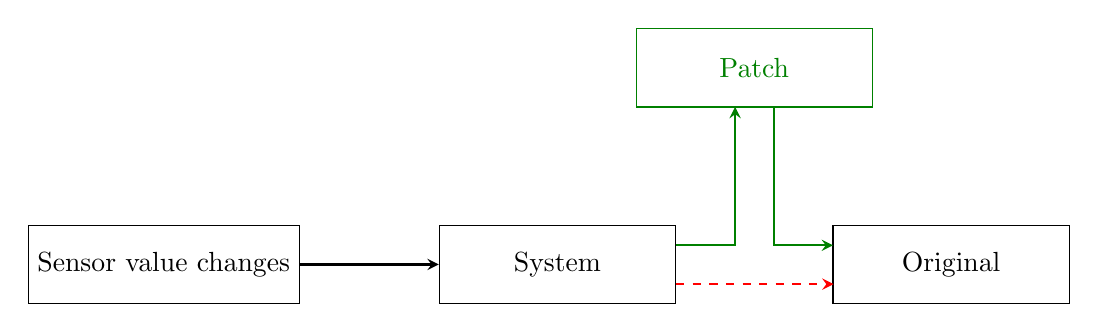
\begin{tikzpicture}
    \tikzstyle{process} = [rectangle, minimum width=3cm, minimum height=1cm, text centered, draw=black]

    \node (sensor) [process] at (0,0) {Sensor value changes};
    \node (system) [process] at (5,0) {System};
    \node (patch) [process, black!50!green] at (7.5,2.5) {Patch};
    \node (function) [process] at (10,0) {Original};

    \draw [thick, ->, >=stealth] (sensor) -- (system);
    \draw [thick, ->, >=stealth, red, dashed] (system.east)+(0,-0.25) -- +(2,-0.25);
    \draw [thick, ->, >=stealth, black!50!green] (system.east)+(0,0.25) -| +(0.75,2);
    \draw [thick, ->, >=stealth, black!50!green] (patch.south)+(0.25,0) |- +(1,-1.75);
  \end{tikzpicture}
  \caption{The function calls from the system are intercepted by our patch and forwarded after modification to the original function.}
  \label{fig:patch}
\end{figure}

\section{Noise Generation}
\label{sec:noise_gen}
\begin{equation}
  value_{new} = \frac{(value_{old} - offset_{sensor})}{gain_{sensor}}
  \label{eq:noise_gen}
\end{equation}

To create the noise, we employ a formula (\ref{eq:noise_gen}) adapted from a study by \citeauthor{DBLP:conf/ndss/DasBC16} \cite{DBLP:conf/ndss/DasBC16}.
This approach leverages established principles of data obfuscation to effectively introduce variability into the sensor readings.
The parameters for offset and gain are chosen within specific ranges determined by that study, ensuring that the introduced noise is effective in obfuscating the sensor data.

The formula works by first subtracting an offset value from the original sensor reading and then dividing the result by a gain factor.
These offset and gain parameters are dynamically adjusted within their predefined ranges to introduce a degree of randomness while preserving the overall utility of the sensor data.
This method ensures that each sensor reading is slightly altered in a way that makes it difficult to reproduce the exact original values, thereby preventing the creation of a consistent and reliable fingerprint.
By carefully selecting the offset and gain ranges, we achieve a balance between data obfuscation and practical usability.
The dynamic adjustment of these parameters allows for consistent randomization of the sensor readings, disrupting attempts to generate a stable fingerprint from the data.
This technique aligns with methods demonstrated in previous research, enhancing the variability of sensor outputs to safeguard against fingerprinting attempts.

The added noise ensures that the sensor values received by the application are not consistent over time, thereby preventing the creation of a stable and persistent fingerprint.
Through this approach, we can enhance the privacy and security of Android users by obfuscating the sensor data in a way that preserves the application's functionality while mitigating the risks associated with sensor fingerprinting.
The reliance on the \verb|SensorEventListener| and its \verb|onSensorChanged| method provides a clear and effective point of intervention, allowing us to implement our countermeasures within the existing Android framework.

Our patch also addresses an important issue when applied to the APKs of mobile browsers.
As mobile browsing is widely used, the integration of sensor functionalities into these browsers raises concerns regarding privacy and security.
With sensors accessible through web technologies like JavaScript, websites can collect sensor data without explicit user consent, potentially leading to unauthorized data collection and privacy infringements.
By extending the protective measures of our patch to mobile browser APKs, we ensure comprehensive mitigation of sensor fingerprinting across all channels of sensor data access on Android devices.
This broader approach strengthens the overall security framework by protecting not only native applications but also web-based interactions.
It offers users increased control over their sensor data, thereby reinforcing digital privacy and reducing the risk of unauthorized data collection across various platforms.

\section{Loss of Precision}
\label{sec:loss_of_precision}
One notable disadvantage of this privacy-enhancing patch is that applications which rely heavily on highly accurate sensor values may suffer in performance. For instance, apps that are controlled by very fine movements, such as precision-based gaming applications, detailed motion tracking software, or certain fitness and health monitoring tools, require exact sensor readings to function optimally. 
The introduction of noise to the sensor data can lead to a degradation in the app's responsiveness and accuracy, resulting in a less satisfactory user experience for those particular applications. However, this trade-off is mitigated by providing users with the choice of whether or not to apply this privacy enhancement.
Users are empowered to decide if they prefer to prioritize their privacy and accept a potential reduction in the accuracy and usability of specific apps, or if they wish to maintain the original performance of these applications at the expense of increased vulnerability to fingerprinting.
This approach allows individuals to make informed decisions based on their specific needs and privacy concerns, balancing the trade-offs between enhanced privacy and app functionality.

Recognizing the need for a balance between privacy protection and the functional requirements of certain apps, one potential solution is the implementation of a custom permission system. 
This system could allow specific applications to request direct access to unaltered sensor data, bypassing the obfuscation introduced by the patch, on the user’s demand, without the need of reinstalling the unpatched version of the software.
This permission system would need to be designed with strict controls to ensure that only trusted applications, which genuinely require precise sensor data, are granted this level of access. 
Users would be able to review and approve these permissions, giving them full control over which apps can access accurate sensor data and under what circumstances.

The custom permission could be integrated into the patch, providing a new layer of security and user control. 
When an application requests access to direct sensor data, the system could prompt the user with a detailed explanation of why the app needs this access and the potential privacy implications. 
Users would then have the option to grant or deny the request based on their understanding and comfort level.

Developers seeking access to direct sensor data would need to adhere to rigid guidelines.
This system would create a transparent and accountable framework for managing sensor data access, providing users with both the protection they need and the functionality they expect from their applications.

\chapter{Implementation}
\label{chap:implementation}
The code ensures the effective obfuscation of sensor data to protect against fingerprinting while maintaining the usability of the application. 
These functions include an intercept method, a noise generating function, and a random value generation function. 
Together, they introduce controlled randomness into the sensor readings, thereby disrupting attempts to create a stable and consistent fingerprint based on the sensor data.

\paragraph{Intercept Method.}
\label{par:intercept_method}
This function, shown in Appendix \ref{lst:intercept_method}, serves as the central hub of the patch, responsible for applying noise to the sensor data.
The intercept method is designed to replace the calls made to sensor-related functions within the application. 
When a sensor reading is requested, the intercept method activates, replacing the original function call that retrieves the sensor data.
The intercept method then calls the noise generating function to alter the sensor data before passing it back to the original function. 
By doing so, the intercept method ensures that any sensor data read by the application is appropriately obfuscated, thereby preventing the formation of consistent and reliable fingerprints.

\paragraph{Noise Generating Function.}
\label{par:noise_gen_func}
The primary role of the noise generating function is to apply the calculated noise to the sensor data, effectively masking the original readings, displayed in \ref{lst:noise_gen_func}.
This function operates by receiving the original sensor values intercepted by the intercept method and then modifying these values according to the predefined algorithm. 
The noise generating function is crucial in balancing privacy protection with usability, ensuring that the altered sensor data remains practical for legitimate application use.

\paragraph{Random Value Generation Function.}
\label{par:random_vale_gen_func}
The random value generation function (\ref{lst:value_gen_func}) underpins the entire noise generation process by providing the random values needed to obfuscate the sensor data.
This function is designed to generate random numbers within specific ranges, which are determined by the type of sensor being accessed.
The random value generation function ensures that each sensor reading is unique and unpredictable, making it significantly more difficult for malicious actors to correlate readings and generate a consistent fingerprint.
The generated random values are then used by the noise generating function to alter the original sensor data.
By continuously producing new random values, this function guarantees that the noise applied to the sensor data varies with each reading, thereby enhancing the overall effectiveness of the privacy protection mechanism.

\paragraph{}
Together, these methods form the basis for our sensor data obfuscation. 
The intercept method acts as a gatekeeper, ensuring that every sensor reading passes through the noise generation process.
The noise generating function applies the necessary modifications to the sensor data, leveraging the random values produced by the random value generation function to introduce controlled variability.
This ensures that the sensor data read by an application is sufficiently obfuscated to mitigate fingerprinting attempts while maintaining the functionality required for legitimate uses.

\paragraph{Application of Patch}
\label{par:applying}
The application of our patch is designed to be straightforward and user-friendly.
It requires an installed Java runtime, along with the precompiled patch and the A2P2 framework, and the APK of the application to be patched.
This simplicity ensures that even those with limited technical expertise can implement the patch without difficulty.

\chapter{Evaluation}
\label{chap:evaluation}
The following sections assesses our methodology in terms of functionality, effectiveness, and usability. 
For testing we selected an APK, focusing particularly on applications that heavily utilize sensor data.
By selecting such applications, we can effectively assess the impact of the patch on sensor data integrity and the overall performance of the app.
This APK serves as a robust testbed for validating the effectiveness of our patch in obfuscating sensor data and preventing fingerprinting.
By conducting tests on applications with high sensor data dependency, we can evaluate both the privacy enhancements introduced by our patch and its practical implications on everyday app usage.
This evaluation ensures that our solution not only enhances user privacy but also preserves the essential functions of the applications tested.

First, the functionality of the patch is validated through a process involving its application to an app called \citetitle{SensorBox}~\cite{SensorBox}, which is designed to gather sensor measurements.
In order to test not only the functionality but also the effectiveness of the patch we created a simple data gathering app~\cite{sensorprint} to collect unaltered and altered data at the same time. 
During the evaluation period, the app collects a significant amount of sensor data, which is then split into two distinct sets: a training dataset and a test dataset.
These recorded values are fed into a machine learning algorithm \cite{DBLP:journals/tifs/AmeriniBCMN17}.
The training dataset is utilized to train a k-nearest neighbors (knn) or random forest classification algorithm, which are standard methods for assessing the variation of data points.
By training the algorithms on the modified sensor data, we aim to evaluate how effectively the introduced noise disrupts the unique patterns of the sensor data and prevents accurate fingerprinting.
We apply gridsearch to determine the best possible parameters for the highest accuracy.
The test dataset is subsequently used to validate the trained algorithm, allowing us to measure the classification accuracy and determine whether the patch has successfully reduced fingerprintability.
The recorded precision quantifies the proportion of correctly predicted positive instances relative to the total number of positive predictions made by the model.
A higher precision value indicates a lower rate of false positives, reflecting better prediction accuracy for positive classifications.
The resulted recall value evaluates the model's ability to identify all relevant instances, with higher values indicating fewer false negatives.
The f1-score provides a harmonic mean of precision and recall, offering a balanced metric that accounts for both false positives and false negatives.
This validation process provides crucial insights into the effectiveness of the patch in enhancing sensor data privacy while maintaining a balance with the functionality of the app.
Through this evaluation, we can ensure that the patch introduces the necessary privacy protections.

\section{Testing}
\label{sec:testing}
Our testing process involved around ten devices running various versions of Android from 10 to the latest current release of Android 14.
We applied the patch to each device and monitored its impact on sensor data handling.
By selecting devices with different hardware configurations we ensured a comprehensive evaluation.
We recorded sensor values from the accelerometer and gyroscope over extended periods to assess the influence of the patch.
Additionally, we tested various applications to understand how the noise added to sensor data affected functionality and user experience.

\subsection{Functionality}
\label{subsec:functionality}
To evaluate the applicability of the patch to existing applications, we selected the simple app \citetitle{SensorBox} as a test case.
The purpose of this test was to determine whether \citetitle{SensorBox} could successfully receive and process the modified sensor values generated by the applied update.
Upon implementing the patch, we observed that \citetitle{SensorBox} seamlessly integrated the patched values without encountering any errors or operational issues.
This successful application demonstrates the compatibility of the patch with established applications and suggests its potential for broader adoption in similar mobile software, particularly those reliant on sensor data.

\begin{figure}[h]
  \centering
  \captionsetup{justification=centering}
  \begin{subfigure}[b]{0.49\textwidth}
    \centering
    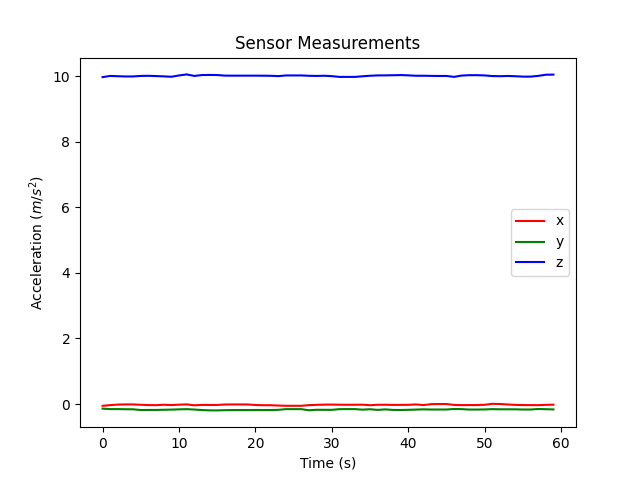
\includegraphics[width=\textwidth]{figures/SensorValuesBefore.png}
    \caption{Values before the patch}
  \end{subfigure}
  \hfill
  \begin{subfigure}[b]{0.49\textwidth}
    \centering
    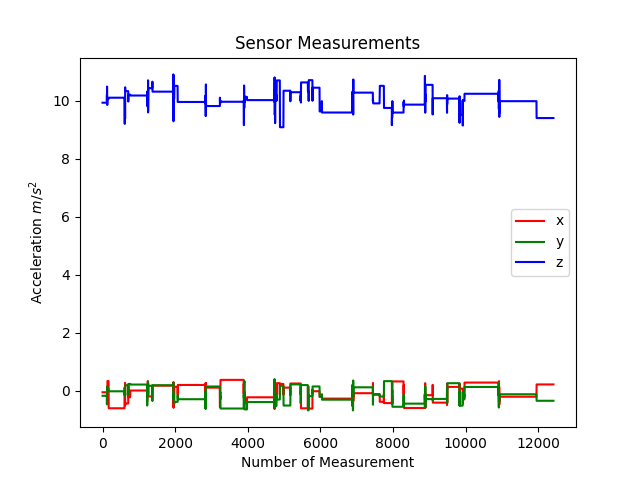
\includegraphics[width=\textwidth]{figures/SensorValuesAfter.png}
    \caption{Values after the patch}
  \end{subfigure}
  \caption{Acceleration sensor values measured before and after the application of the patch on the same device.}
  \label{fig:values}
\end{figure}

\subsection{Effectiveness}
\label{subsec:effectiveness}
To conduct this test, sensor values from the accelerometer and gyroscope were recorded over the duration of a minute.
This experiment aimed to observe how the patch influenced the consistency of sensor data captured by the application.
By analyzing the recorded data, we could determine the extent to which the patch successfully obfuscated the sensor values.
Comparing the consistency of the sensor readouts before and after applying the patch, a significant change can be observed in Figure \ref{fig:values}, mirroring the findings of previous research studies. 
Before the application of our patch, the sensor values exhibit a high degree of consistency, which can be exploited for fingerprinting.
However, after the patch introduces randomization and noise, the sensor readouts become visibly less consistent as it is visualized in Figure \ref{fig:knn_decision_boundaries}.

\begin{figure}[h!]
  \centering
  \captionsetup{justification=centering}
  \begin{subfigure}[b]{0.49\textwidth}
    \centering
    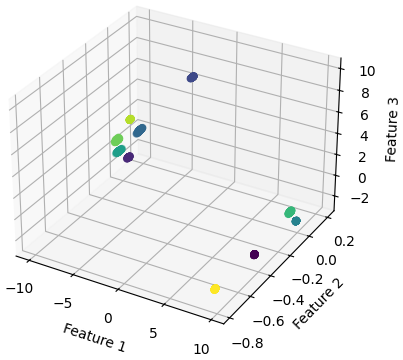
\includegraphics[width=\textwidth]{figures/knn_before.png}
    \caption{knn decision boundaries\\before applying noise}
  \end{subfigure}
  \hfill
  \begin{subfigure}[b]{0.49\textwidth}
    \centering
    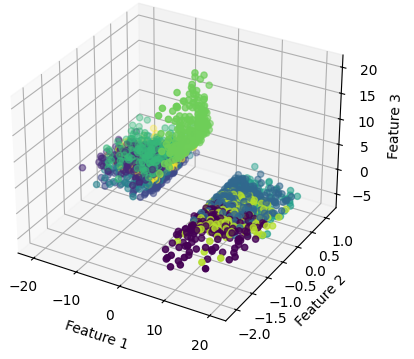
\includegraphics[width=\textwidth]{figures/knn_after.png}
    \caption{knn decision boundaries\\after applying noise}
  \end{subfigure}
  \caption{3D visualization of knn decision boundaries.}
  \label{fig:knn_decision_boundaries}
\end{figure}

When the classification algorithm used the unpatched, unmasked data it was able to associate all of the devices with their measurement with 100\% confidence.
After applying the patch and retraining the algorithm it was only able to match the devices with 72.916\% accuracy, even with our few samples of ten devices as shown in Figure \ref{tab:knn_results}. 
When analyzing the classification results for each individual device, it becomes clear that the performance metrics all declined, except one, from their previous values of 100\% as shown in Figure \ref{tab:knn_detailed_results}.
This reduction highlights a shift in the effectiveness of our fingerprinting method when applied to devices after being patched, making it more difficult to maintain a consistent fingerprint across different devices.

The observed drop in these metrics indicates that the classifier's ability to distinguish device-specific patterns has been compromised.
This is due to the introduced variability by our patch in sensor data across devices.
Our results demonstrate a low incidence of false positives, indicating a high degree of confidence in the classification of the observed instances.
Notably, this level of accuracy was maintained even when distinguishing between devices of the same make and model, underscoring the robustness and reliability of this simple fingerprinting approach.
These findings suggest that the model is capable of effectively identifying subtle differences between devices, even when hardware and software configurations are largely identical.

We believe that this accuracy would decrease even more with the use of a lot more devices, increasing the disruption of consistent error values.
This disruption in the data stability effectively hinders the ability to create a reliable fingerprint, aligning with the results documented in other papers.
This observed change underscores the effectiveness of the patch in enhancing privacy by preventing the formation of stable and persistent sensor-based identifiers.

\begin{table}[h]
  \centering
  \captionsetup{justification=centering}
  \subfloat{
    \begin{tabularx}{.175\textwidth}{r|}        
      \\ \hline
      accuracy      \\
      macro avg     \\
      weighted avg  \\
    \end{tabularx}
  }
  \quad
  \subfloat[Results before obfuscation]{
    \begin{tabularx}{.335\textwidth}{|ccc|}
      precision & recall & f1-score \\ \hline
                &        & 1.00     \\
      1.00      & 1.00   & 1.00     \\
      1.00      & 1.00   & 1.00     \\
    \end{tabularx}
  }
  \quad
  \subfloat[Results after obfuscation]{
    \begin{tabularx}{.335\textwidth}{|ccc|}
      precision & recall & f1-score \\ \hline
                &        & 0.73     \\
      0.73      & 0.73   & 0.73     \\
      0.73      & 0.73   & 0.73     \\
    \end{tabularx}
  }
  \caption{The performance outcomes of the knn classifier over the test dataset.}
  \label{tab:knn_results}
\end{table}

\begin{table}[h]
  \centering
  \captionsetup{justification=centering}
  \begin{tabular}{r|cccc|}
                        & precision & recall  & f1-score  & support \\ \hline
    Galaxy A34 5G \_01  & 0.82      & 0.66    & 0.73      & 74      \\
    Galaxy A54 5G \_01  & 0.59      & 0.60    & 0.59      & 82      \\
    Galaxy A55 5G \_01  & 0.95      & 0.96    & 0.95      & 76      \\
    Galaxy M23 5G \_01  & 0.44      & 0.37    & 0.40      & 68      \\
    Galaxy M23 5G \_02  & 0.61      & 0.65    & 0.63      & 66      \\
    Galaxy S21 5G \_01  & 0.59      & 0.58    & 0.58      & 76      \\
       Galaxy S23 \_02  & 0.77      & 0.94    & 0.85      & 62      \\
  Galaxy Tab S10+ \_01  & 0.72      & 0.76    & 0.74      & 72      \\
 Galaxy Tab S9 5G \_01  & 0.77      & 0.80    & 0.78      & 75      \\
        Nokia 6.1 \_01  & 1.00      & 1.00    & 1.00      & 69      \\
  \end{tabular}
  \caption{Detailed results of the knn classifier for each individual device.}
  \label{tab:knn_detailed_results}
\end{table}

\pagebreak
\subsection{Usability}
\label{subsec:usability}
The patch was applied to a motion-controlled game \cite{krassesSpiel} to assess its impact on user experience.
This specific test was designed to determine how the introduction of noise to sensor readouts would affect applications that rely heavily on precise sensor data.
When the app was running with the patch installed, the added noise in the sensor readouts caused noticeable shaking of the controlled object.
This unintended side effect made the game more challenging to play, as the smooth and accurate movement necessary for controlling the game object was compromised.
The increased difficulty highlighted the potential trade-offs between enhancing privacy and maintaining the usability of certain types of applications, particularly those that depend on fine-tuned sensor accuracy for optimal performance.

\section{Noise Level Adjustment}
\label{sec:noise_level_adjustment}
Modifying the level of noise applied to sensor data enhances resistance against device fingerprinting, though it presents trade-offs that impact application functionality.
By increasing the noise intensity, it becomes more difficult for fingerprinting algorithms to reliably distinguish unique device signatures as shown in Figure \ref{tab:knn_increased_results}, thereby strengthening user privacy.
In our testing, increasing the gain of the sensor values resulted in a more pronounced decrease in the effectiveness of fingerprinting methods.
This adjustment disrupted the distinctiveness of sensor data, thereby enhancing privacy by making it more challenging for algorithms to identify unique device signatures.
In contrast, modifying the offset applied to the sensor readouts had a relatively limited impact on the fingerprinting process.
The offset adjustment did not significantly alter the underlying characteristics of the sensor data, thus allowing more identifiable patterns to remain detectable. 
However, excessive noise disrupts the accuracy and reliability of sensor data, which many applications rely upon for core functions, rendering them less usable or even unusable.
Conversely, reducing the noise level to preserve application functionality diminishes the effectiveness of fingerprinting protection as demonstrated in Figure \ref{tab:knn_decreased_results}.
Achieving an optimal balance between these competing priorities is thus important.

\begin{table}[h]
  \centering
  \captionsetup{justification=centering}
  \subfloat{
    \begin{tabularx}{.175\textwidth}{r|}        
      \\ \hline
      accuracy      \\
      macro avg     \\
      weighted avg  \\
    \end{tabularx}
  }
  \quad
  \subfloat[Results with high gain]{
    \begin{tabularx}{.335\textwidth}{|ccc|}
      precision & recall & f1-score \\ \hline
                &        & 0.51     \\
      0.52      & 0.52   & 0.52     \\
      0.52      & 0.51   & 0.51     \\
    \end{tabularx}
  }
  \quad
  \subfloat[Results with high gain and offset]{
    \begin{tabularx}{.335\textwidth}{|ccc|}
      precision & recall & f1-score \\ \hline
                &        & 0.41     \\
      0.41      & 0.41   & 0.41     \\
      0.41      & 0.41   & 0.41     \\
    \end{tabularx}
  }
  \linebreak
  \subfloat{
    \begin{tabularx}{.175\textwidth}{r|}        
      \\ \hline
      accuracy      \\
      macro avg     \\
      weighted avg  \\
    \end{tabularx}
  }
  \quad
  \subfloat[Results with default offset and gain]{
    \begin{tabularx}{.335\textwidth}{|ccc|}
      precision & recall & f1-score \\ \hline
                &        & 0.73     \\
      0.73      & 0.73   & 0.73     \\
      0.73      & 0.73   & 0.73     \\
    \end{tabularx}
  }
  \quad
  \subfloat[Results with high offset]{
    \begin{tabularx}{.335\textwidth}{|ccc|}
      precision & recall & f1-score \\ \hline
                &        & 0.54     \\
      0.55      & 0.55   & 0.55     \\
      0.55      & 0.54   & 0.54     \\
    \end{tabularx}
  }
  \caption{knn classifier results after applying the patch with increased noise levels.}
  \label{tab:knn_increased_results}
\end{table}

\begin{table}[h]
  \centering
  \captionsetup{justification=centering}
  \subfloat{
    \begin{tabularx}{.175\textwidth}{r|}        
      \\ \hline
      accuracy      \\
      macro avg     \\
      weighted avg  \\
    \end{tabularx}
  }
  \quad
  \subfloat[Results with low gain]{
    \begin{tabularx}{.335\textwidth}{|ccc|}
      precision & recall & f1-score \\ \hline
                &        & 0.78     \\
      0.79      & 0.78   & 0.78     \\
      0.78      & 0.78   & 0.78     \\
    \end{tabularx}
  }
  \quad
  \subfloat[Results with default gain and offset]{
    \begin{tabularx}{.335\textwidth}{|ccc|}
      precision & recall & f1-score \\ \hline
                &        & 0.73     \\
      0.73      & 0.73   & 0.73     \\
      0.73      & 0.73   & 0.73     \\
    \end{tabularx}
  }
  \linebreak
  \subfloat{
    \begin{tabularx}{.175\textwidth}{r|}        
      \\ \hline
      accuracy      \\
      macro avg     \\
      weighted avg  \\
    \end{tabularx}
  }
  \quad
  \subfloat[Results with low offset and gain]{
    \begin{tabularx}{.335\textwidth}{|ccc|}
      precision & recall & f1-score \\ \hline
                &        & 0.91     \\
      0.91      & 0.91   & 0.91     \\
      0.91      & 0.91   & 0.91     \\
    \end{tabularx}
  }
  \quad
  \subfloat[Results with low offset]{
    \begin{tabularx}{.335\textwidth}{|ccc|}
      precision & recall & f1-score \\ \hline
                &        & 0.81     \\
      0.81      & 0.81   & 0.81     \\
      0.81      & 0.81   & 0.81     \\
    \end{tabularx}
  }
  \caption{knn classifier results after applying the patch with decreased noise levels.}
  \label{tab:knn_decreased_results}
\end{table}

\chapter{Discussion \& Limitations}
\label{chap:disc_and_limits}
During our limited testing, we were unable to test our implementation on a sufficient number of devices to definitively state whether the patch works as intended across a broad spectrum of hardware configurations.
While the initial results were promising, indicating that the patch could successfully obfuscate sensor data and disrupt fingerprinting attempts, the limited sample size means that these results cannot be generalized to all devices.
Unfortunately, our access to a diverse range of devices was limited.
This scarcity of devices hindered our ability to perform extensive and comprehensive testing.

Previous studies have often introduced additional, artificially derived features to improve the reliability and accuracy of fingerprinting techniques \cite{DBLP:journals/popets/DasBC18, DBLP:journals/tifs/ZhangBS21}.
By contrast, our approach was tested solely by training our algorithm on the combined raw sensor readouts, without incorporating any supplementary, artificially generated or preprocessed features.
This methodology allows for a direct assessment of the effectiveness of our approach based purely on the available sensor data.
Consequently, our results provide insights into the potential of raw sensor readouts alone to serve as a basis for fingerprinting, in contrast to methods that rely on additional feature engineering to enhance accuracy.

The patch was tested in a limited laboratory setting, which did not sufficiently simulate real-world scenarios.
During our testing, the device remained stationary on a table, which does not reflect the dynamic conditions under which mobile devices typically operate.
This controlled environment allowed us to focus on the fundamental aspects of the patch functionality without the interference of external factors. 
However, it also means that the testing did not account for variables such as user movement or environmental changes. 
Consequently, the results obtained from this limited testing environment may not fully represent the performance of the patch in real-world usage.

Despite the limited scope of our testing, we are still convinced of the results of previous studies that state noise generation is a successful method for mitigating fingerprinting.
These studies provide a solid foundation for our approach, demonstrating that introducing variability into sensor data can effectively prevent the creation of consistent and identifiable fingerprints.
We are confident in the robustness of our patch design and the alignment of our methods with those proven effective in existing research.

While the obfuscated sensor data generated by our patch enhances privacy by disrupting fingerprinting attempts, it does impact the accuracy of sensor readings. 
To address the needs of applications that rely on precise sensor data, a custom permission system could be used, allowing specific apps to access direct sensor data under controlled and user-approved conditions. 
This approach balances the importance of both privacy protection and functional accuracy, ensuring that users retain control over their data while enabling high-precision applications to operate effectively.


\chapter{Conclusion}
\label{chap:conclusion}
Fingerprinting devices based on sensor value imperfections poses a significant privacy concern, as these subtle errors, often caused by manufacturing variances or environmental factors, can be exploited to uniquely identify and track devices.
Unlike traditional identifiers, sensor-based fingerprints do not require explicit user permissions, making them a covert and persistent threat to user anonymity. 

Our approach addresses the problem of consistent sensor error values which can be used for fingerprinting.
We intercept sensor readouts with the help of the A2P2 framework and manipulate them with added noise.
After limited testing, which showed promising tendencies, we conclude that it is feasible to protect against fingerprinting based on the unique built-in errors of sensors by masking these errors with randomly generated noise.

By introducing artificial noise, the distinctive patterns and unique characteristics that these sensors typically exhibit become harder to identify, which complicates efforts to track or profile devices.
This method not only enhances privacy but also maintains the integrity of sensor data for general use, ensuring that the overall functionality of the device is not heavily compromised.
While the added noise effectively disrupts fingerprinting efforts, it simultaneously degrades the accuracy and reliability of the sensor data.
Excessive noise can impair many applications depending on accurate sensor data for activities such as navigation, environmental monitoring, or gesture recognition, reducing user experience and the app's practical utility.
Thus, while noise augmentation can provide privacy benefits, it must be carefully balanced against the need to maintain the operational effectiveness of applications.

Furthermore, implementing an additional permission for apps to access unobfuscated sensor data, could allow the user to grant explicit consent on demand, ensuring that user experience is not compromised for applications requiring precise sensor measurements.
By offering this user-controlled flexibility, we could ensure that critical applications can operate without degradation in performance while still protecting against potential privacy breaches.
This combined strategy of noise generation and user-controlled permissions provides a comprehensive and balanced solution, enhancing privacy without sacrificing the functionality and accuracy required by essential applications. 
Through this approach, we can significantly increase the difficulty for adversaries attempting to create a consistent fingerprint of devices based on the sensors used. 

%--- INDEX and BIBLIOGRAPHY ----------------------------------------------------

%% Print List of Acronyms and Symbols  (optional)
%\printnoidxglossary[title={Notation}]
%\printnoidxglossary[type=acronym]

% Print bibliography and include it in the table of contents:
\printbibliography[heading=bibintoc]

\appendix

\chapter{Appendix}
\label{chap:appendix}

% \section{Code Snippets}
% \label{sec:code_snippets}

\begin{lstlisting}[language=java, caption=Interception Helper Methods, label=lst:intercept_help_method]
/**
* Checks if a PatchListener is already associated with the SensorEventListener received.
* Creates new one of not or binds additional sensors to the existing ones.
* @param listener the original SensorEventListener instance.
* @param sensor the Sensor the listener should receive values from.
* @see SensorEventListener
* @see Sensor
* @see PatchListener
* @return return custom PatchListener object containing the original listener.
*/
private static SensorEventListener addListener(SensorEventListener listener, Sensor sensor) {
  PatchListener plistener = PATCH_MAPPINGS.stream().filter(pl -> pl.getListener().equals(listener)).findAny().orElse(new PatchListener(listener));
  plistener.sensors.add(sensor);
  PATCH_MAPPINGS.add(plistener);
  return plistener;
}

/**
* Finds the PatchListener is already associated with the SensorEventListener
* received and removes the sensor it is unregistering from.
* Removes the PatchListener if no more Sensors are bound to it.
* @param listener the original SensorEventListener object.
* @param sensor the Sensor the listener should receive values from.
* @see SensorEventListener
* @see Sensor
* @see PatchListener
* @return return custom PatchListener object containing the original listener. If none found it returns the original listener
*/
private static SensorEventListener removeListener(SensorEventListener listener, Sensor sensor) {
  PatchListener plistener = PATCH_MAPPINGS.stream().filter(pl -> pl.getListener().equals(listener)).findAny().orElse(null);
  if (plistener == null) return listener;
  if (sensor != null) plistener.sensors.remove(sensor);
  else plistener.sensors.clear();
  if (plistener.sensors.isEmpty()) return PATCH_MAPPINGS.remove(PATCH_MAPPINGS.indexOf(plistener));
  return plistener;
}
\end{lstlisting}

\begin{lstlisting}[language=java, caption=Intercept Methods, label=lst:intercept_method]
/**
* Intercepts the function call to this function and
* calls it with the custom PatchListener wrapper for the original.
* @see SensorManager
* @see PatchInstanceMethod
* @see OriginalMethods
* @return value from original registerListener method
*/
@PatchInstanceMethod
public static boolean registerListener(SensorManager sm, SensorEventListener listener, Sensor sensor, int samplingPeriodUs) {
  return OriginalMethods.android_hardware_SensorManager.registerListener(sm, addListener(listener, sensor), sensor, samplingPeriodUs);
}

/**
* Intercepts the function call to this function and
* replaces the SensorEventListener object with the registered PatchListener
* before calling the original function.
* @see SensorManager
* @see PatchInstanceMethod
* @see OriginalMethods
*/
@PatchInstanceMethod
public static void unregisterListener(SensorManager sm, SensorEventListener listener) {
  OriginalMethods.android_hardware_SensorManager.unregisterListener(sm, removeListener(listener, null));
}
\end{lstlisting}
\pagebreak
\begin{lstlisting}[language=java, caption=Noise Generating Function, label=lst:noise_gen_func]
/**
* Selects offset and gain for the appropriate sensor and
* applies noise to the value if the right sensor is read.
* @param event SensorEvent.
* @see SensorEvent
*/
private void manipulateValues(SensorEvent event) {
  float offset = Utils.getOffset(event.sensor.getType());
  float gain = Utils.getGain(event.sensor.getType());

  switch(event.sensor.getType()) {
    case Sensor.TYPE_ACCELEROMETER:
    case Sensor.TYPE_GYROSCOPE:
      event.values[AXIS_X] = applyNoise(event.values[AXIS_X], offset, gain);
      event.values[AXIS_Y] = applyNoise(event.values[AXIS_Y], offset, gain);
      event.values[AXIS_Z] = applyNoise(event.values[AXIS_Z], offset, gain);
      break;
    default:
      break;
  }
}
\end{lstlisting}

\begin{lstlisting}[language=java, caption=Random Value Generation Function, label=lst:value_gen_func]
/**
* Applies noise to the original sensor value.
* @param original Original sensor value.
* @param lambda_offset +/- offset to be applied to the original value.
* @param lambda_gain 1 +/- gain to be applied to the original value.
* @return float obscured sensor value.
*/
private float applyNoise(final float original, final float lambda_offset, final float lambda_gain) {
  float offset = generateRandomValue(0 - Math.abs(lambda_offset), 
                                           0 + Math.abs(lambda_offset));
  float gain = generateRandomValue(1 - Math.abs(lambda_gain), 
                                         1 + Math.abs(lambda_gain));
 
  return (original - offset) / gain;
}
\end{lstlisting}
\pagebreak
\begin{lstlisting}[language=java, caption=SensorEventListener Methods, label=lst:patchlistener]
/**
  * Implements the abstract method from the SensorEventListener.
  * Calls the same function of the original listener after manipulating the received SensorEvent and passes is down.
  * @see SensorEventListener
  * @see SensorEvent
  * @see Patch
  */
@Override
public void onSensorChanged(SensorEvent event) {
    Patch.manipulateValues(event);
    listener.onSensorChanged(event);
}

/**
  * Implements the abstract method from the SensorEventListener.
  * Calls the same function of the original listener passes down the received parameters.
  * @see SensorEventListener
  * @see Sensor
  */
@Override
public void onAccuracyChanged(Sensor sensor, int accuracy) {
    listener.onAccuracyChanged(sensor, accuracy);
}
\end{lstlisting}
\pagebreak
\begin{lstlisting}[language=python, caption=Classifier Function, label=lst:classifier]
def classify(path: str,
  classifier: str = 'knn',
  gridsearch: bool = True
  ) -> KNeighborsClassifier | RandomForestClassifier:
  """
  Loads the data of the given directory and trains a knn classification algorithm, 
  then tests the accuracy. 

  Args:
    path (str): Folder containing the directories with the CSV files.
    classifier (str): Selected classifier method.
    gridsearch (bool): Should the parameters for the model be optimised via gridsearch 
                  or use default ones.

  Returns:
    Classifier: model trained on the dataset.
  """
  x, y = load_data(path)

  x_train, x_test, y_train, y_test = train_test_split(
  x, y, test_size=0.3, random_state=42)

  model = None
  param_grid = None

  if classifier == 'knn':
    param_grid = {
      'n_neighbors': [1, 2, 5],
      'weights': ['uniform', 'distance'],
      'algorithm': ['auto', 'ball_tree', 'kd_tree', 'brute']
    }
    model = KNeighborsClassifier(
      algorithm='auto', n_neighbors=1, weights='uniform')
  elif classifier == 'rf':
    param_grid = {
      'n_estimators': [200, 250, 300],
      'max_depth': [30, 40, 50]
    }
    model = RandomForestClassifier(n_estimators=250, max_depth=40)

  if gridsearch:
    if param_grid is None:
      raise ValueError("Parameters for GridSearch are not set.")

    grid_search = GridSearchCV(model, param_grid, cv=5, scoring='accuracy')
    grid_search.fit(x_train, y_train)
    best_model = grid_search.best_estimator_
  else:
    best_model = model

  if best_model is None:
    raise ValueError("Model is not set.")

  y_pred = best_model.predict(x_test)

  print("Accuracy:", accuracy_score(y_test, y_pred))
  print("Best Parameters:", best_model.get_params())
  print("")
  print(classification_report(y_test, y_pred))

  return best_model
\end{lstlisting}

\end{document}
